%%%%%%%%%%%%%%%%%%%%%%%%%%%%%%%%%%%%%%%%%%%%%%%%%%%%%%%%%%%%%%%%%%%%%%%%%%%%%%%%%%%%%%%%%%%%%%%%%%%%%%
%
%   Filename    : chapter_4.tex 
%
%   Description : This file will contain your Research Methodology.
%                 
%%%%%%%%%%%%%%%%%%%%%%%%%%%%%%%%%%%%%%%%%%%%%%%%%%%%%%%%%%%%%%%%%%%%%%%%%%%%%%%%%%%%%%%%%%%%%%%%%%%%%%

\chapter{Research Methodology}

This chapter outlines the methodological framework adopted to achieve the research objectives. As illustrated in Figure~\ref{fig:methodology-pipeline}, the research process is structured as a dual-stream pipeline composed of two interrelated tracks: one focused on model development and instance segmentation, and the other on the design, deployment, and testing of a crowdsourcing platform. While these tracks proceed in parallel, they are tightly integrated—converging at later stages for the automated annotation of crowdsourced media and final dataset construction.

The upper stream encompasses data sourcing, manual annotation, and model fine-tuning, while the lower stream represents the iterative development and testing phases of the WeCyclePH platform. Together, they enable the transformation of raw user-contributed media into a geospatially structured dataset. Each stage of this dual-process methodology is detailed in the sections that follow.

\begin{figure}[!htbp]
    \centering
    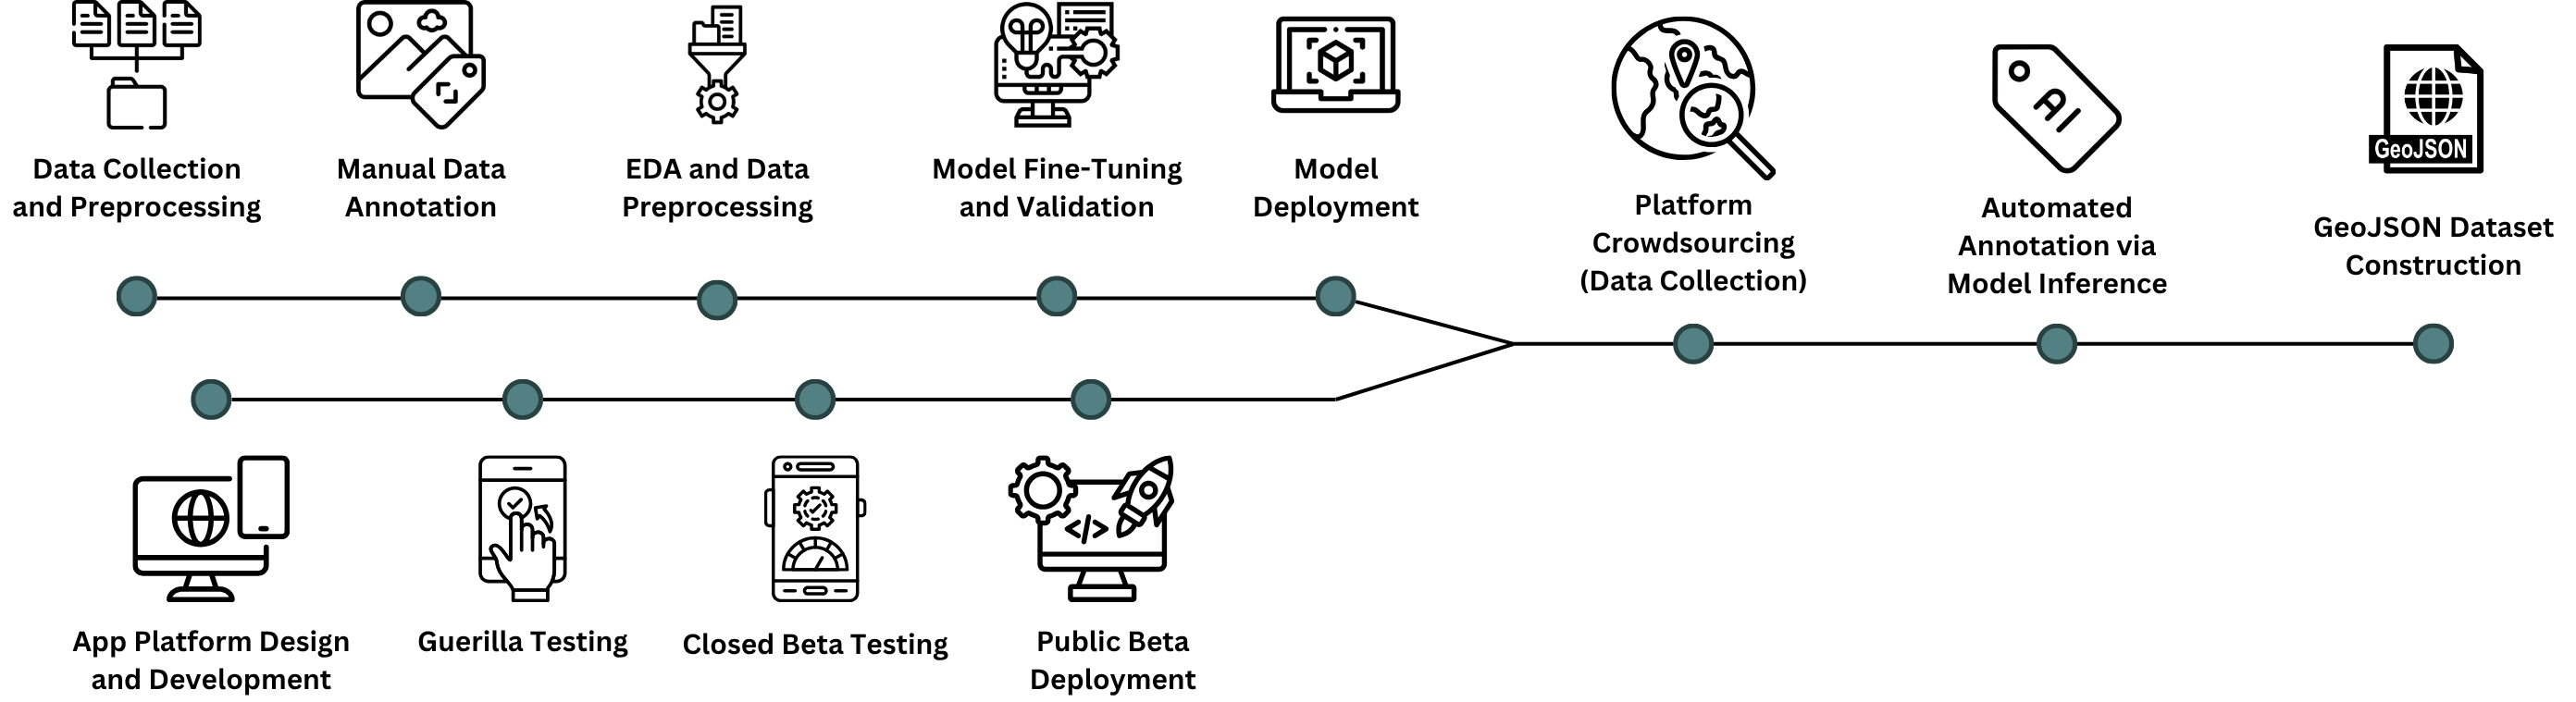
\includegraphics[width=1\linewidth]{figures/chapt4/methodology-pipeline.png}
    \caption{Dual-stream project pipeline of WeCyclePH, illustrating the parallel development of the mobile application for data crowdsourcing.}
    \label{fig:methodology-pipeline}
\end{figure}

\section{Training the Instance Segmentation Model}

This section outlines the end-to-end process of developing and deploying a YOLOv11-based instance segmentation model tailored for analyzing urban cycling environments in Metro Manila. It details the workflow from data collection and preprocessing, manual annotation, and exploratory data analysis to model fine-tuning, evaluation, and deployment. By integrating publicly sourced POV cycling videos, rigorous annotation protocols, and targeted augmentation strategies, the study adapts a state-of-the-art segmentation architecture to detect both common urban road users and context-specific cycling infrastructure. The following subsections describe each stage in the pipeline, ensuring methodological transparency and reproducibility.

\subsection{Data Collection and Preprocessing}

To develop a robust instance segmentation model for analyzing urban cycling environments, video data was sourced primarily from publicly available YouTube content. The selected videos featured front-facing point-of-view (POV) cycling vlogs recorded along major roads in Metro Manila, offering a first-hand perspective of real-world conditions and dynamic interactions within and around bicycle lanes. These videos were chosen based on their ability to capture critical infrastructure elements, such as dedicated bike lanes, traffic signs, pedestrian crossings, road markings, and common obstructions, ensuring a comprehensive representation of the target object classes in various urban contexts.

Before inclusion in the dataset, all videos underwent a quality assurance process to ensure visual clarity, resolution consistency, and relevance to the study objectives. A custom pre-processing pipeline was implemented to automate the download process and standardize video resolution to 720p. Each video was then segmented into 5-second intervals, which were subsequently decomposed into individual frames. This step transformed the continuous video footage into a large collection of still images, allowing for more granular and manageable data annotation.

The extracted frames were imported into the Computer Vision Annotation Tool (CVAT), where manual annotation was conducted to label key objects and environmental features. These annotations serve as ground truth for training the instance segmentation model, enabling it to learn and accurately recognize diverse objects encountered in urban cycling environments.

All video data were obtained in compliance with the terms of service, copyright regulations, and usage policies of their respective platforms. The research team adhered to ethical data handling standards, with particular attention paid to privacy and intellectual property considerations. All materials were used strictly for academic and non-commercial research purposes.

\subsection{Manual Data Annotation}

The custom dataset used in this study was manually annotated using the Computer Vision Annotation Tool (CVAT), an open-source platform for image and video annotation. Researchers manually labeled each frame extracted from the video segments to identify key objects relevant to urban cycling. These include critical infrastructure elements such as bike lane markings, cyclist-specific traffic signals, bollards, and other road features that affect cycling conditions.

Beyond infrastructure, annotations also covered a wide range of urban objects such as pedestrians, motor vehicles (e.g., cars, motorcycles, trucks, buses, jeepneys, and tricycles), and traffic-related structures. CVAT's polygon segmentation tools enabled precise, multi-label annotations that capture the spatial complexity of these objects within each frame.

Each object was annotated using polygon masks and tagged with class labels, ensuring detailed, context-aware data for training the YOLOv11 instance segmentation model. This approach enhances the model's capacity to detect and track multiple object types across successive frames in user-generated cycling videos.

\begin{figure}[h!]
    \centering
    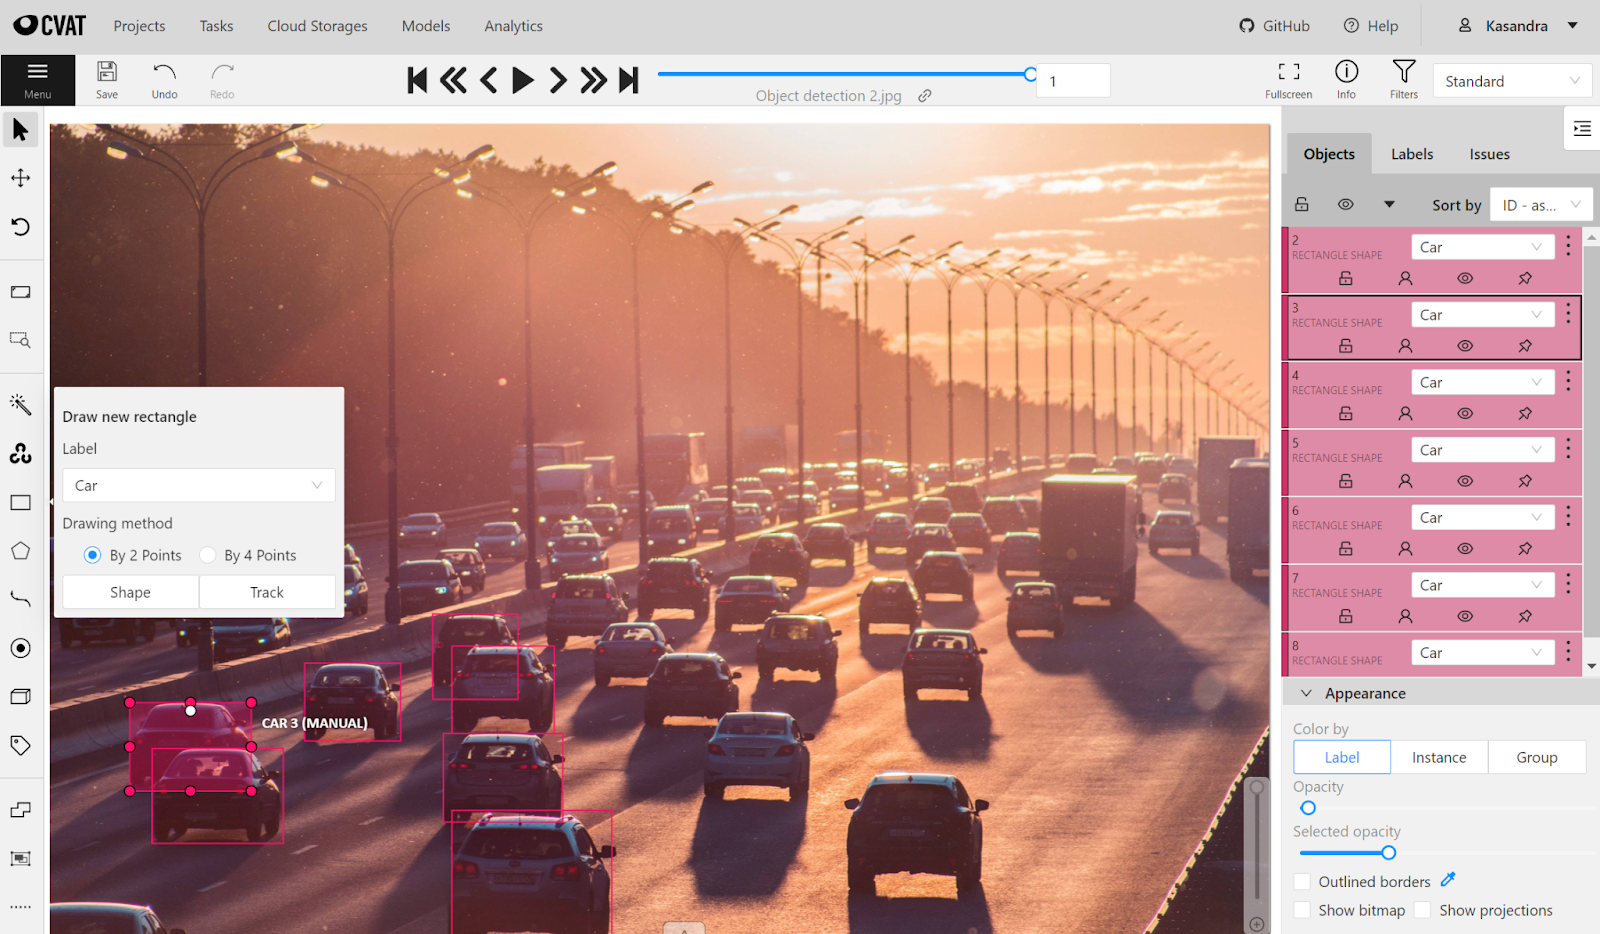
\includegraphics[width=0.75\linewidth]{figures/cvat_annotate.png}
    \caption{CVAT interface used for annotating urban cycling scenes.}
    \label{fig:cvat_annotation}
\end{figure}

To support model training, ten critical object classes were identified based on their relevance to bicycle lane assessment and urban road safety. The inclusion of these classes allows the model to monitor lane use, detect obstructions, and identify rule violations that may impact cyclists.

Table~\ref{tab:combined_classes} summarizes these classes along with example images from the dataset.



% Then replace your table block with this:
\begin{longtable}{|c|l|p{6cm}|}
\caption{Defined object classes with descriptions and representative images.}
\label{tab:combined_classes}
\\ \hline
\textbf{Image} & \textbf{Class} & \textbf{Description} \\ \hline
\endfirsthead

\hline
\textbf{Image} & \textbf{Class} & \textbf{Description} \\ \hline
\endhead

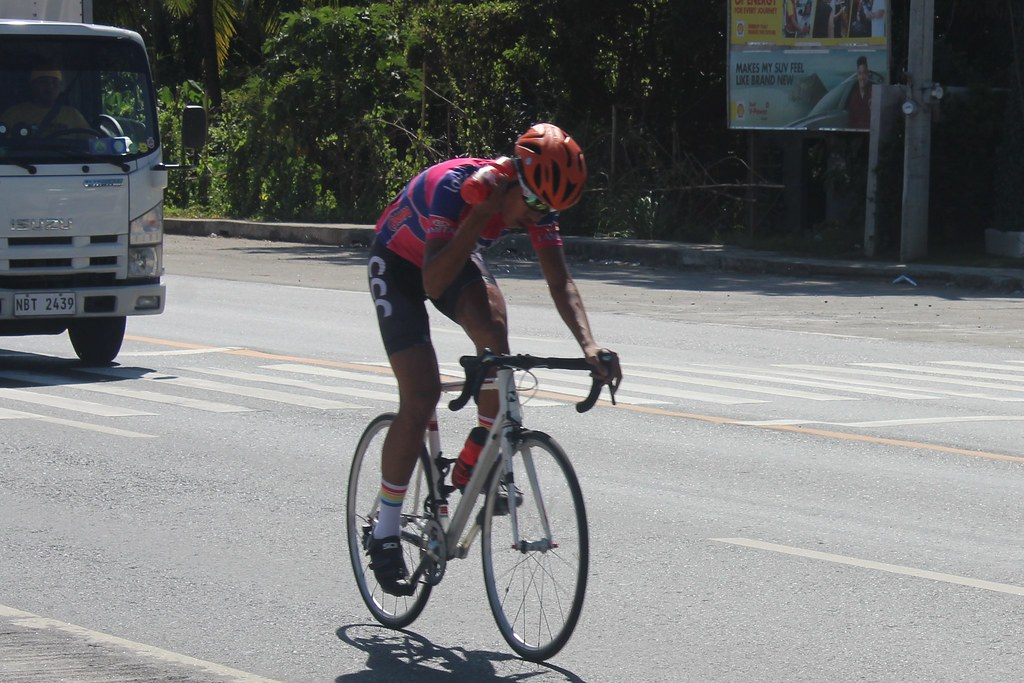
\includegraphics[width=2.5cm]{figures/cyclist_class.jpg} & \texttt{bicycle} & Bicycles on the road, representing cyclists. \\ \hline
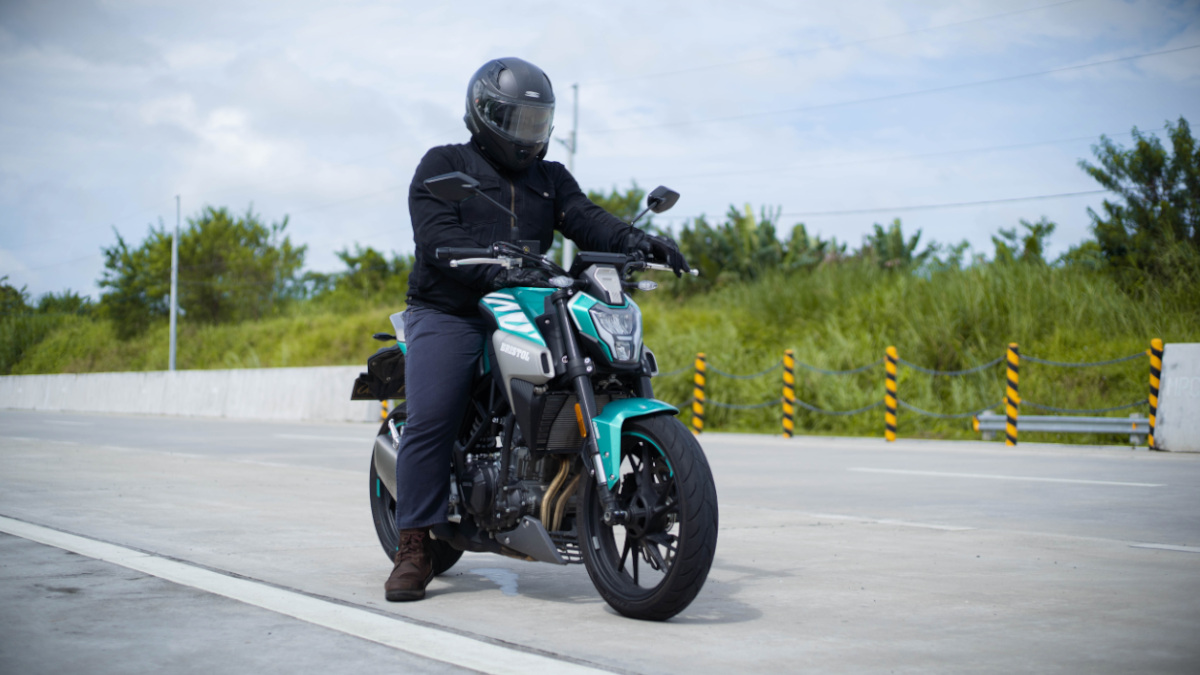
\includegraphics[width=2.5cm]{figures/motorcyclist_class.jpg} & \texttt{motorcycle} & Two-wheeled motorized vehicles. \\ \hline
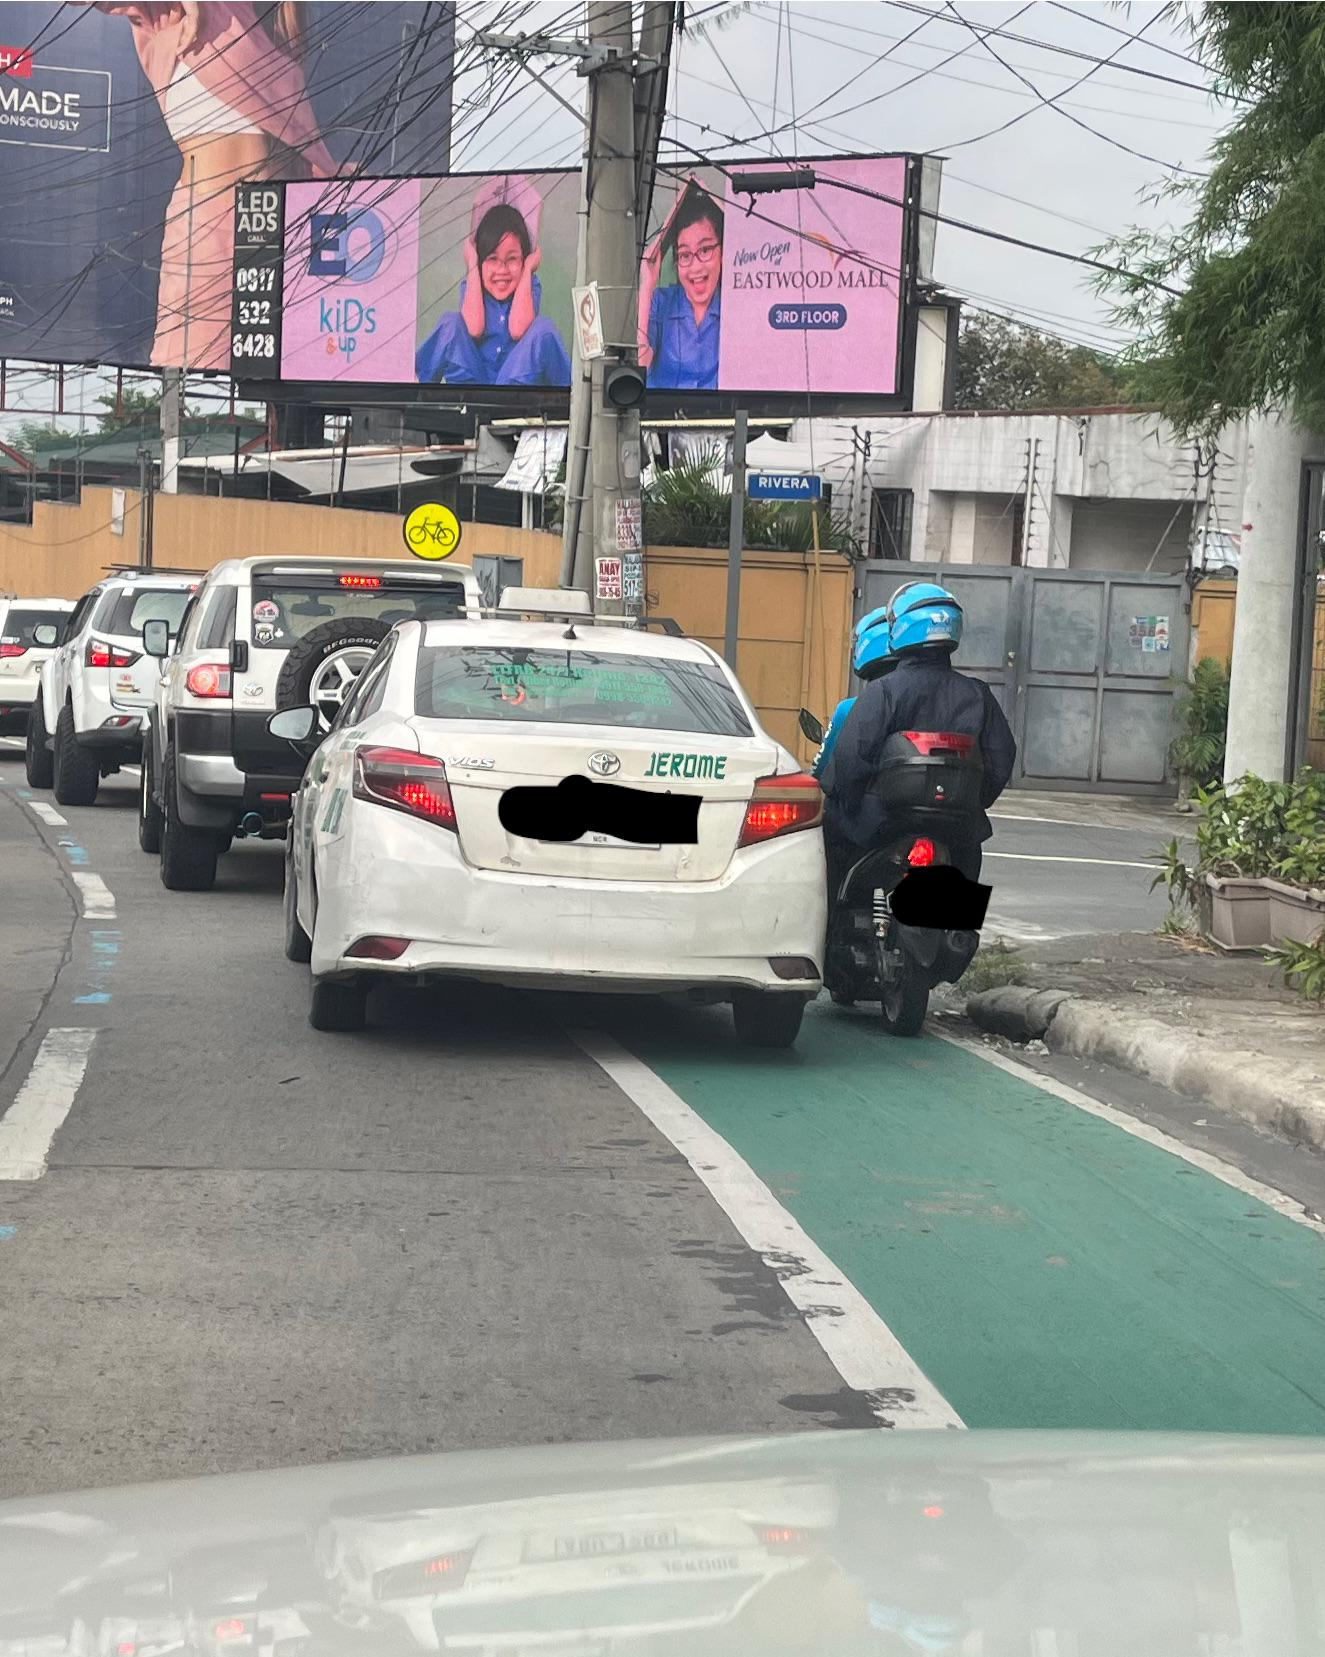
\includegraphics[width=2.5cm]{figures/car_class.jpg} & \texttt{car} & Small to medium-sized four-wheeled vehicles. \\ \hline
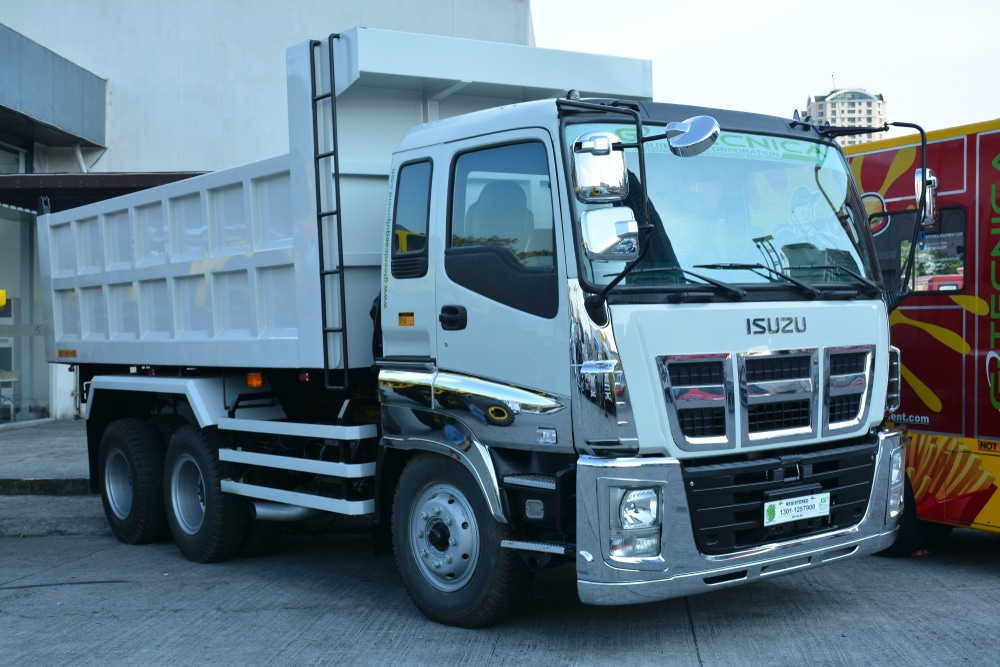
\includegraphics[width=2.5cm]{figures/truck_class.jpg} & \texttt{truck} & Larger motorized vehicles such as delivery trucks. \\ \hline
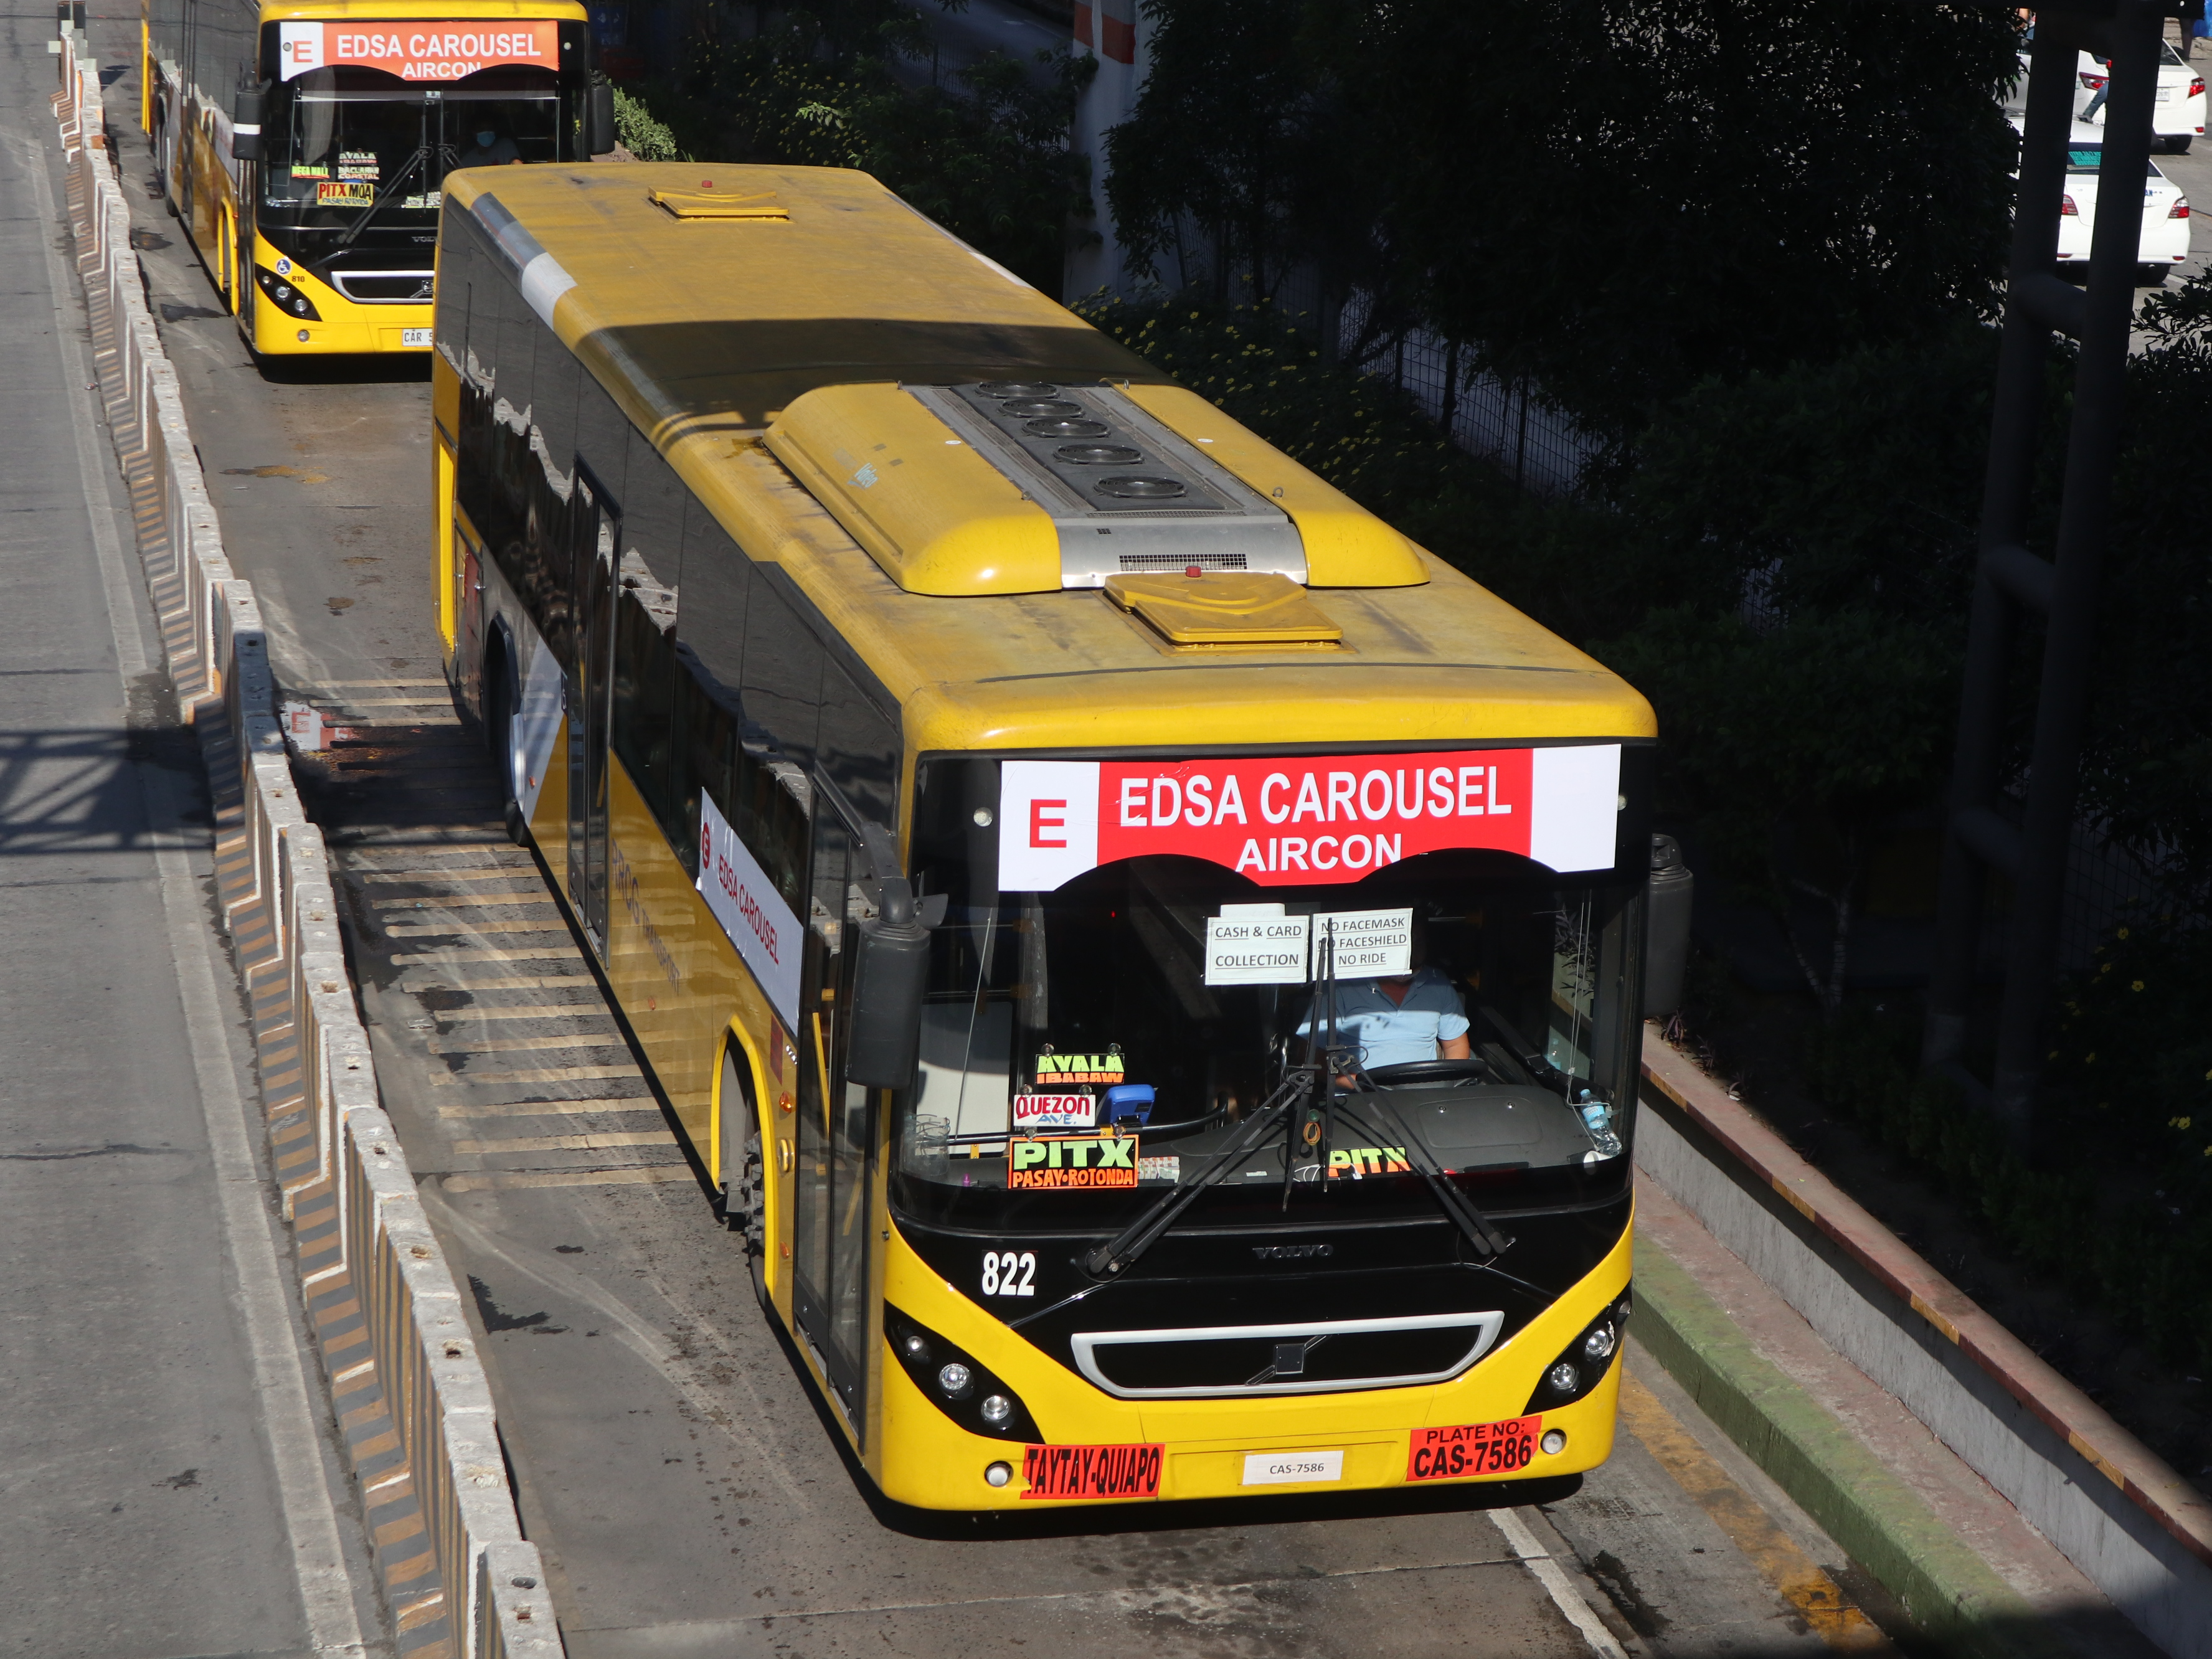
\includegraphics[width=2.5cm]{figures/bus_class.jpg} & \texttt{bus} & Public transport buses. \\ \hline
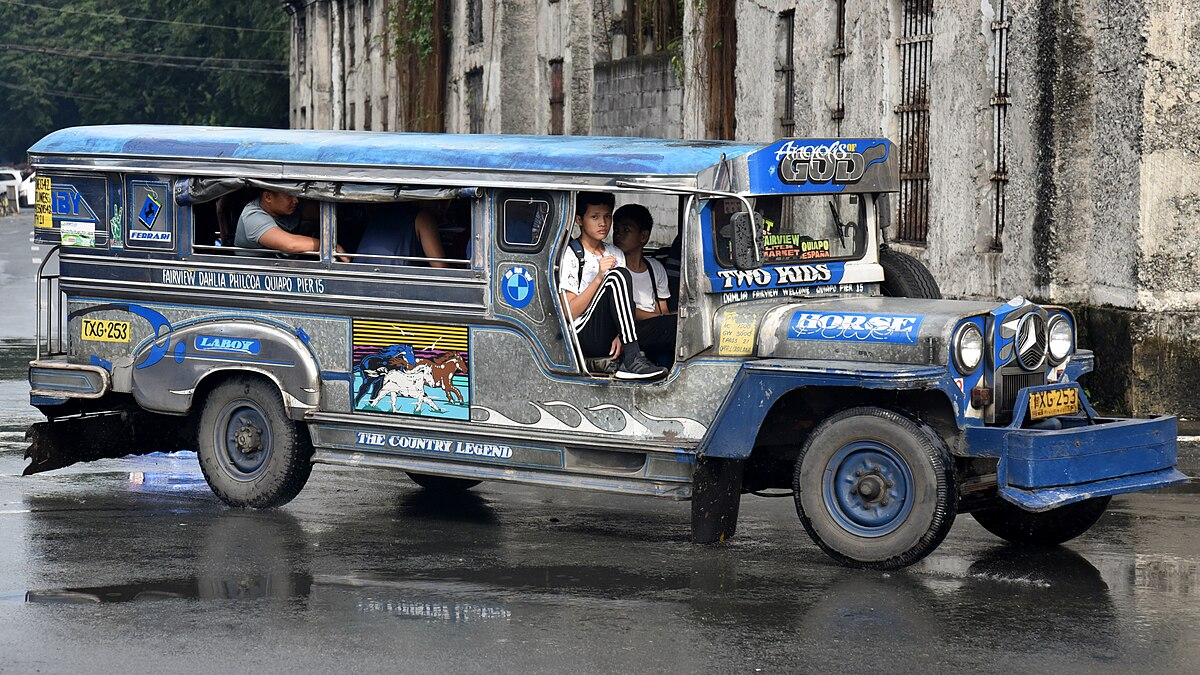
\includegraphics[width=2.5cm]{figures/jeepney_class.jpg} & \texttt{jeepney} & Public utility vehicles specific to the Philippines. \\ \hline
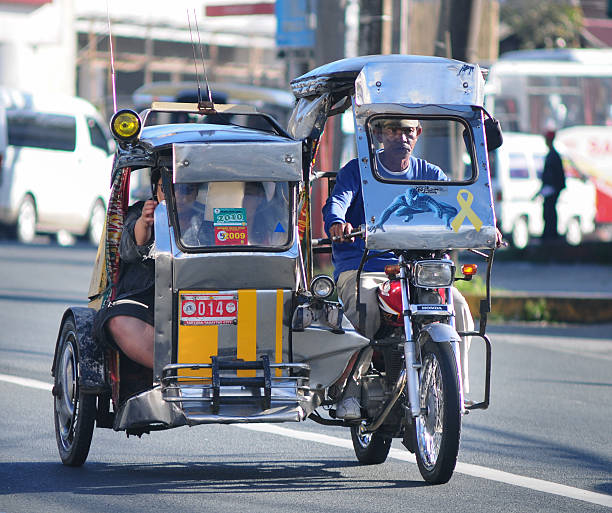
\includegraphics[width=2.5cm]{figures/tricycle_class.jpg} & \texttt{tricycle} & Three-wheeled vehicles common in the Philippines. \\ \hline
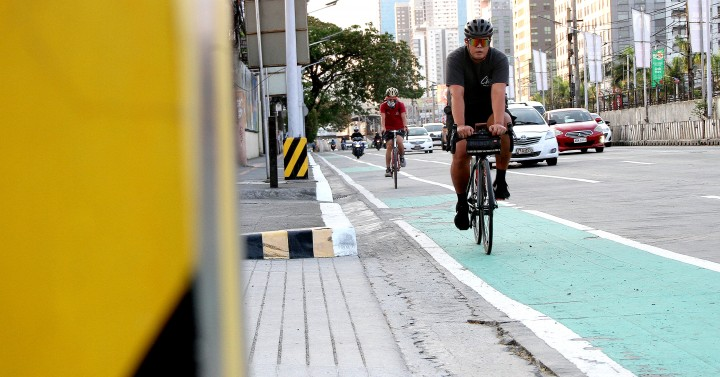
\includegraphics[width=2.5cm]{figures/lane_markings_class.jpg} & \texttt{bike\_lane} & Painted lines or signage designating bike lanes. \\ \hline
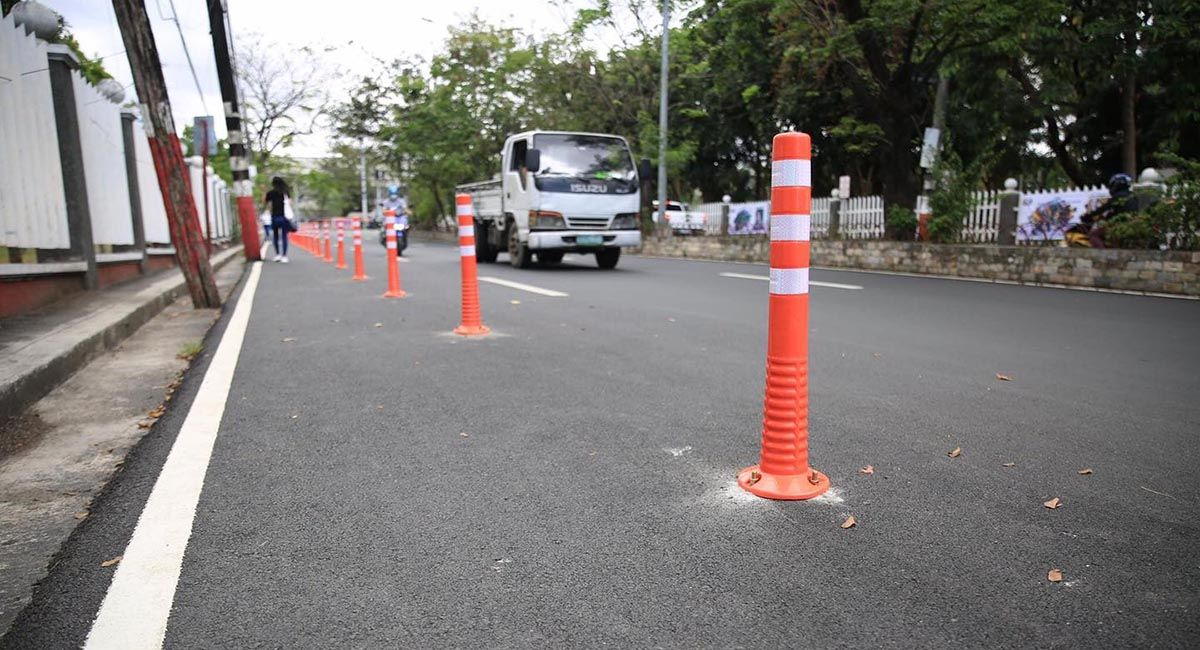
\includegraphics[width=2.5cm]{figures/bollards_class.jpeg} & \texttt{barrier} & Physical dividers such as bollards, cones, or barriers. \\ \hline
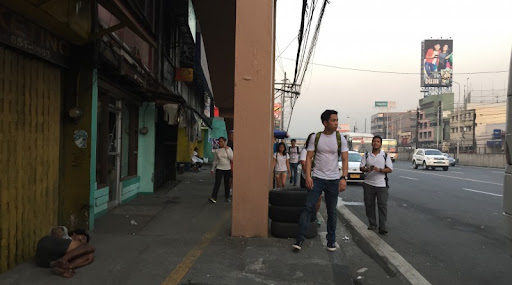
\includegraphics[width=2.5cm]{figures/pedestrian_class.jpg} & \texttt{person} & Individuals walking, jogging, or crossing near bike lanes. \\ \hline

\end{longtable}


The annotation strategy was guided by performance metrics such as mean Average Precision (mAP) and Intersection over Union (IoU). Annotation efforts were expanded only when new samples improved either metric by at least \textbf{0.5}, ensuring resource efficiency and performance-driven dataset refinement.

On average, each image contained approximately \textbf{5 to 10 annotated instances}, reflecting the dense and complex nature of urban cycling environments where multiple objects often overlap within a single frame.


\subsection{EDA and Data Preprocessing}

\subsubsection{Data Splitting and Preparation}

After completing the annotation process, the dataset was divided into training, validation, and test sets following a standard \textbf{70-15-15 split}. This partitioning supports the systematic training and evaluation of the instance segmentation model.

\paragraph{Training Set (70\%).} This subset was used to train the YOLOv11 model, providing it with a wide variety of annotated cycling-specific instances to learn object features and segmentation patterns.

\paragraph{Validation Set (15\%).} The validation set was used during model development for hyperparameter tuning, such as learning rate and batch size adjustment. It ensured model optimization while guarding against overfitting.

\paragraph{Test Set (15\%).} The test set was reserved for final performance evaluation, providing an unbiased assessment of the model's accuracy and generalization capability on previously unseen data.

\subsubsection{Class Imbalance and Undersampling}

To address the issue of class imbalance across annotated object instances, undersampling was applied to ensure equal representation of all classes during training. Table~\ref{tab:initial_class_counts} shows the original instance distribution across classes.

\begin{table}[h]
\centering
\begin{tabular}{l r}
\toprule
\textbf{Class} & \textbf{Original Instance Count} \\
\midrule
car & 986 \\
tricycle & 146 \\
truck & 173 \\
bicycle & 362 \\
motorcycle & 545 \\
bike\_lane & 697 \\
barrier & 636 \\
bus & 43 \\
person & 234 \\
jeepney & 144 \\
\bottomrule
\end{tabular}
\caption{Initial object instance counts prior to undersampling.}
\label{tab:initial_class_counts}
\end{table}

To ensure balance, a minimum threshold of 43 instances (equal to the rarest class, \texttt{bus}) was set for all classes. A total of 194 label files were retained after per-class undersampling, ensuring that each object class had at most 43 labeled instances. This technique prevents the model from being biased toward overrepresented classes during training.

\subsubsection{Duplicate Image Filtering via Perceptual Hashing}

To improve dataset quality and prevent redundancy, perceptual hashing was applied using the \texttt{imagehash} library to detect and remove exact and near-duplicate images.

\begin{itemize}
    \item \textbf{Total images processed:} 7,540
    \item \textbf{Unique images:} 4,829 (64.05\%)
    \item \textbf{Exact duplicates:} 1,833 (24.31\%)
    \item \textbf{Augmented duplicates:} 703 (9.32\%)
\end{itemize}

This step ensured the model would not overfit on repeated or low-variability data and promoted learning from a diverse and unique image set.

\subsubsection{Data Augmentation}

To further enrich the dataset and improve generalization, several augmentation techniques were applied to the training images. These included:

\begin{itemize}
    \item Horizontal flipping
    \item 90-degree rotation
    \item Gaussian blur
    \item Color jitter
    \item Shadow simulation
\end{itemize}

As a result, the training set achieved a more balanced object instance distribution, as shown in Table~\ref{tab:augmented_class_counts}.

\begin{table}[h]
\centering
\begin{tabular}{l r}
\toprule
\textbf{Class} & \textbf{Post-Augmentation Count} \\
\midrule
car & 1,561 \\
tricycle & 1,337 \\
truck & 896 \\
bicycle & 1,386 \\
motorcycle & 1,561 \\
bike\_lane & 1,561 \\
barrier & 1,561 \\
bus & 1,561 \\
person & 560 \\
jeepney & 1,561 \\
\bottomrule
\end{tabular}
\caption{Object instance counts in the training set after data augmentation.}
\label{tab:augmented_class_counts}
\end{table}

These augmentation techniques not only increased the size of the training set but also introduced variations in lighting, orientation, and appearance—improving the model's robustness in real-world deployment scenarios.

\subsection{Model Fine-Tuning and Validation}

The instance segmentation model training phase leverages a pre-trained YOLOv11 model trained on the COCO 2017 dataset. This pretraining provides the model with feature extraction capabilities for detecting a wide range of general objects. To adapt the model to the specific context of urban cycling and Philippine road environments, it was fine-tuned using a custom dataset. This dataset consists of annotated frames from user-generated videos, focusing on infrastructure elements, road conditions, and objects relevant to local cycling experiences. This fine-tuning ensures that the model can accurately recognize both globally relevant objects and context-specific features unique to the study's focus.

\subsubsection{Model Selection}
The YOLOv11 model was selected for its demonstrated efficacy in real-time object detection and segmentation tasks, particularly within constrained environments such as bicycle lanes. As highlighted by \citet{GarciaPajuelo2024}, YOLO architectures consistently achieve superior performance in detecting vehicles and other objects in urban contexts, conditions that closely align with the objectives of this study.

\textbf{Existing Detection Capabilities:} YOLOv11 was pre-initialized on the COCO dataset, enabling it to detect a wide range of objects relevant to urban environments. These include:
\begin{itemize}
    \item \textit{Vehicles:} Cars, motorcycles, buses, and trucks, which frequently interact with or encroach upon bicycle lanes.
    \item \textit{Pedestrians:} Individuals walking near or crossing bike lanes, a common occurrence in urban areas.
    \item \textit{Road Signs:} Standard traffic signs, including those for pedestrians and vehicles.
\end{itemize}

These capabilities make YOLOv11 well-suited for general urban object detection. However, its existing pre-trained weights were not optimized for the unique context of cycling and Philippine roads.

\textbf{Limitations in Cycling and Philippine Road Contexts:} 
Despite its advanced capabilities, YOLOv11 faces notable limitations in the following areas:
\begin{itemize}
    \item \textit{Bike Lane-Specific Elements:} The model was not pre-trained to detect objects unique to bicycle lanes, such as bike lane markers, bollards, or bicycle-specific signals. These objects were critical for evaluating bike lane usability and safety.
    \item \textit{Localized Infrastructure:} Philippine-specific road elements, such as informal street vendor carts, tricycles (three-wheeled motorized vehicles), and utility posts, were not commonly included in pre-trained datasets.
    \item \textit{Road Obstructions:} Obstructions like potholes, construction debris, and other informal barriers frequently encountered on Philippine roads were challenging for the model without additional training.
    \item \textit{Cyclists:} While the model can detect people, it does not differentiate between pedestrians and cyclists without fine-tuning or additional class definitions.
\end{itemize}

To address these limitations, this study fine-tuned the YOLOv11 model on a custom dataset annotated specifically for bicycle lane environments in the Philippines. By integrating new annotations for bike lane markers, tricycles, street vendor carts, and localized road hazards, the model was adapted to better suit the unique urban cycling context in this region. The goal was to enable the model to detect and interpret objects that significantly impact bicycle lane usability and safety.

This tailored approach ensures that the YOLOv11 model not only leverages its pre-trained strengths but also accounts for the nuances of cycling and road conditions specific to the Philippines.

YOLOv11 was initialized using weights pre-trained on the COCO-seg dataset, a comprehensive benchmark dataset containing detailed annotations for object segmentation across 80 diverse categories. This pretraining phase enables the model to leverage a robust and generalized feature extraction capability, significantly accelerating the convergence process during fine-tuning and reducing the dependency on extensive training data. By utilizing the knowledge gained from COCO-seg, the model was adapted to detect and classify domain-specific objects pertinent to urban cycling environments, including cyclists, vehicles, road signs, and lane markers.

The architecture of YOLOv11 has been optimized to balance precision and computational efficiency, making it particularly suitable for segmenting objects in real-time applications. Its ability to process high-resolution input data with minimal latency ensures its relevance for analyzing dynamic lane interactions, where timely and accurate detection was essential. To further tailor the model to the specific requirements of this study, hyperparameters such as batch size, learning rate, and anchor box dimensions were systematically adjusted. These refinements aim to enhance the model's segmentation accuracy and tracking reliability, particularly in dense and complex urban cycling scenarios.


\subsubsection{Training Process}
The training process consists of a multi-step pipeline designed to optimize the performance of YOLOv11 using the annotated training dataset. Following the techniques proposed by \citet{Neven:2018}, we configured the training parameters with a batch size of 16 and an initial learning rate of 0.001. This learning rate was adjusted dynamically based on feedback from the model and the characteristics of the dataset. Training was conducted for a maximum of 100 epochs, with early stopping criteria based on validation loss to mitigate overfitting. Throughout the process, the validation set was utilized to fine-tune hyperparameters, enhancing the model's precision and recall. This iterative process ensures the model effectively learns object boundaries and distinguishes between classes.

Upon completing training, the model's instance segmentation capabilities were deployed in real-time on video data. During deployment, the model was integrated with a tracking algorithm to maintain object identities across consecutive frames. This tracking capability allows the model to consistently monitor objects such as cyclists, vehicles, and lane features as they move through the scene, preventing double-counting. This temporal continuity was crucial for analyzing dynamic lane usage patterns. The tracking module operates independently during video execution, enabling the model to evaluate interactions without requiring additional training steps.

The object tracking capability was essential for analyzing video data and maintaining consistent identities for objects across different frames. However, it functions independently of the crowdsourcing application. This separation allows the crowdsourcing platform to concentrate on efficient data collection, while more computationally intensive tasks, such as instance segmentation and tracking, were handled offline.

\subsubsection{Evaluation Metrics}
The performance of the model was assessed using a suite of metrics that measure segmentation accuracy, detection reliability, and tracking consistency. Drawing from the framework established by \citet{GarciaPajuelo2024}, the evaluation utilizes key metrics, including accuracy, precision, and recall, to quantify the model's effectiveness in detecting and segmenting objects within the lanes. Intersection over Union (IoU) and mean Average Precision (mAP) were employed to measure segmentation accuracy, particularly focusing on the overlap between predicted and actual object boundaries. This was crucial for identifying compliance within lane boundaries. For tracking evaluation, Multi-Object Tracking Accuracy (MOTA) and the ID Switch Count, as outlined in \citet{Neven:2018}, were utilized to measure the model's ability to maintain object identities across frames. Together, these metrics provide a comprehensive assessment of the model's capability to detect, segment, and track multiple objects within the dynamic environment of urban bicycle lanes.


\subsection{Model Deployment}

Upon completion of training and validation, the final instance segmentation model was deployed using the Ultralytics HUB platform. Ultralytics HUB is a cloud-based environment designed for managing, testing, and deploying YOLO-based models, offering seamless integration for experimentation and inference at scale.

The model was exported in the appropriate YOLO format and uploaded to the HUB, where it could be accessed via an intuitive web interface. This deployment enabled centralized model hosting, version control, and performance monitoring, making it easier to share results and conduct live testing on new image or video inputs.

Deploying to Ultralytics HUB also facilitated rapid iteration and model accessibility for both research and potential field deployment. It allowed the research team to perform real-time inference on unseen data, visualize segmentation masks directly on video frames, and evaluate how well the model generalized to cycling environments beyond the training dataset.

This deployment marks the final stage in the model development pipeline, ensuring that the trained YOLOv11 instance segmentation model is accessible, testable, and scalable for future use cases involving cyclist experience analysis and urban mobility assessment.

\section{Building the Crowdsourcing Platform: WeCyclePH}

This section details the design, development, and implementation of WeCyclePH, the crowdsourcing platform developed to collect, organize, and enrich cyclist-contributed data. The platform was conceptualized to empower cyclists to document their experiences in real time and post-ride through mobile and web interfaces. By combining GPS tracking, video capture, and manual annotation features, the system facilitates the collection of both quantitative and qualitative data reflecting the conditions of urban and semi-urban cycling environments. This section outlines the strategies used to design user-friendly and technically robust applications, the development methodologies adopted to ensure rapid iteration and functional completeness, and the architectural decisions that underpin the system's scalability, reliability, and data integrity.

\subsection{Initial Prototype}

The initial prototype was created to validate the feasibility of the core concept: enabling cyclists to record their rides, annotate their experiences, and contribute to a shared repository of cycling data. At this stage, two essential features were implemented. The first was GPS-based trip recording, modeled after Strava, which logged the route, distance, duration, and other ride statistics in real time. The second was a video-based annotation workflow inspired by editing software such as CapCut. This system allowed users to upload a video of their trip and then select specific segments within the video on which to place annotations.

A central assumption in this design was that the videos uploaded by users would represent their entire cycling trips, from start to finish. This assumption shaped the annotation workflow, which relied on continuous video playback to give users the ability to navigate the timeline and mark events—such as road hazards, infrastructure conditions, or points of interest—at the exact moments they occurred. By requiring that annotation take place after the ride, rather than during it, the prototype was intended to minimize distractions and ensure the safety of cyclists.

The primary objectives for testing this prototype were to determine whether first-time users could intuitively operate the core features, to identify any significant usability barriers, and to assess whether the video-segment annotation approach was both practical and engaging for contributors.

\subsubsection{Participants}
Participants were recruited opportunistically from the cycling community in Batangas and Metro Manila. Locations included coffee shops frequented by cyclists, organized cycling events, and public gathering spots for riders. Any cyclist willing to test the application for a short period of time qualified for inclusion. No demographic filtering was applied at this stage; the goal was to observe interactions from a broad and naturally occurring user sample. Refer to Table \ref{tab:GuerillaTesting_Demographic} for the participant demographic.


\begin{table}[H]
\centering
\renewcommand{\arraystretch}{1.3}
\begin{tabular}{|
>{\raggedright\arraybackslash}p{1.2cm}|
>{\raggedright\arraybackslash}p{0.8cm}|
>{\raggedright\arraybackslash}p{3.2cm}|
>{\raggedright\arraybackslash}p{4cm}|
>{\raggedright\arraybackslash}p{3.8cm}|
}
\hline
\textbf{Gender} & \textbf{Age} & \textbf{Regular Biker?} & \textbf{Primary Location} & \textbf{Used Cycling Apps While Riding?} \\
\hline
Male & 19 & Yes & Tanauan, Batangas & No \\
\hline
Male & 23 & Yes & Tanauan to Malvar, sometimes goes on long cycling trips & Yes \\
\hline
Male & 23 & I bike, but only rarely & Tanauan & No \\
\hline
Male & 19 & I bike, but only rarely & Tanauan, Sto. Tomas & No \\
\hline
Male & 23 & I bike, just seldomly & Tanauan to Malvar & Yes \\
\hline
Female & 22 & I bike, but only rarely & Lipa & No \\
\hline
Male & 23 & I bike, just seldomly & Quezon City, Metro Manila & Yes \\
\hline
Male & 21 & I bike, but only rarely & Makati, Metro Manila & No \\
\hline
Female & 20 & I bike, but only rarely & Taguig & No \\
\hline
Male & 21 & I bike, just seldomly & Tanauan, Batangas & No \\
\hline
\end{tabular}
\caption{Demographic profile of guerrilla testing participants, detailing their gender, age, cycling frequency, primary location, and use of cycling applications while riding, showing that most were male, based in Batangas, and infrequent cyclists with limited experience using cycling apps.}
\label{tab:GuerillaTesting_Demographic}
\end{table}


\subsubsection{Setup and Distribution}

The prototype was built for Android devices and installed on a project-owned smartphone used exclusively for testing. The decision to limit testing to a provided device ensured a consistent technical environment, removing variables such as device performance or storage limitations from early evaluations. Guerilla testing was conducted in public settings without formal scheduling, replicating the conditions under which a casual user might download and use the application without prior instruction.

\subsubsection{Testing Procedure}

The planned testing method for the initial prototype was guerilla testing, selected for its ability to produce rapid, authentic feedback. Participants were introduced to the application with minimal explanation and asked to perform one to three tasks:

\begin{itemize}
    \item Record a ride using the GPS tracking feature.
    \item Upload a video representing the ride.
    \item Annotate specific events by selecting and marking segments within the uploaded video.
\end{itemize}

The researcher observed the interaction closely, providing clarification only after the participant had attempted the task. Each session lasted between 5 and 15 minutes, allowing for multiple short trials within a single day of testing.

\subsubsection{Feedback Collection}
Feedback was gathered immediately after each session through short verbal debriefs. Observational notes were recorded in real time using Google Forms, capturing moments of hesitation, errors in navigation, or confusion about the workflow. These qualitative observations were used to identify patterns of difficulty—particularly with video uploads and timeline navigation—that would inform design refinements for the next development stage.

\subsection{Closed Beta}

The closed beta phase was intended to evaluate the platform in a semi-controlled environment, focusing on usability, stability, and feature performance after refinements prompted by guerilla testing. The most significant planned change at this stage was a complete redesign of the annotation workflow. Video uploads were made optional, enabling users to annotate trips without being constrained by the need to upload full-ride footage. Annotations could now be placed directly on GPS-tracked ride segments, and an auto-pause feature was introduced to allow mid-ride annotations without affecting recorded statistics. These changes aimed to address two key pain points observed in the prototype: the technical difficulty of uploading large video files and the tediousness of reviewing an entire video to make multiple annotations.

\subsubsection{Participants}
The participants for this Beta Testing phase were carefully selected based on their cycling experience and engagement with digital cycling tools. The focus was on experienced cyclists who cycle regularly, with a minimum of one ride per week. Three male participants, aged between 18 and 24, were chosen to represent a mix of cycling habits and app usage behaviors.

All three participants had over three years of cycling experience and remain active cyclists. Of these participants, two regularly use digital cycling apps during their rides, such as Strava or similar tools, to track performance and monitor cycling data. The third participant, however, does not use any digital applications for cycling, providing a non-tech user perspective on the app's usability.


\begin{table}[H]
\centering
\renewcommand{\arraystretch}{1.3}
\begin{tabular}{|
>{\raggedright\arraybackslash}p{1.2cm}|
>{\raggedright\arraybackslash}p{0.8cm}|
>{\raggedright\arraybackslash}p{2.5cm}|
>{\raggedright\arraybackslash}p{2.5cm}|
>{\raggedright\arraybackslash}p{2.5cm}|
>{\raggedright\arraybackslash}p{2.5cm}|
>{\raggedright\arraybackslash}p{2.5cm}|
}
\hline
\textbf{ID} & \textbf{Age} & \textbf{Primary Cycling Location} & \textbf{Cycling Frequency} & \textbf{Cycling Experience} & \textbf{Familiarity with Cycling Apps} \\
\hline
CB01 & 23 & Metro Manila & 3x a week & 4 years & Yes \\
\hline
CB02 & 22 & Metro Manila & 3--5x a week & 3 years & Yes \\
\hline
CB03 & 21 & Metro Manila & 2--3x a week & 3 years & Yes \\
\hline
\end{tabular}
\caption{Profile of closed beta cyclist-participants with prior experience using cycling applications, including their age, primary cycling location, riding frequency, and years of cycling experience.}
\label{tab:cyclist_app_users}
\end{table}

\subsubsection{Setup and Distribution}
The Android APK was shared directly with participants via Google Drive. Participants were guided through the sideloading process to install the app on their personal devices. Testing took place in a controlled urban cycling route in Metro Manila, designed to replicate common real-world scenarios such as navigating bike lanes, avoiding road obstructions, and adjusting to varied terrain.

\subsubsection{Testing Procedure}
Each participant took part in a 30-minute supervised test session, during which they recorded a ride, added manual annotations, and optionally uploaded cycling video footage. The session was immediately followed by a 20-minute semi-structured interview to capture initial impressions. Afterward, participants were instructed to complete at least three independent rides over the following days to assess the platform's performance in their regular cycling environments.

\subsubsection{Feedback Collection}
Feedback was collected from two sources: transcribed audio from the post-test interviews and field notes recorded during both supervised and independent usage. These qualitative data sources provided insight into usability, stability, and the likelihood of long-term engagement with the platform.



\subsection{Public Beta}
The Public Beta phase marked the final stage of the WeCyclePH deployment and represented the platform’s transition into real-world cycling environments. This stage followed iterative improvements made during the guerrilla and closed beta testing phases. Unlike earlier evaluations conducted in controlled settings, the public beta involved organic, unsupervised usage by a wider pool of cyclists across Metro Manila and Batangas. Participants accessed the mobile and web applications through open recruitment channels and contributed voluntarily through ride recordings, annotations, and media uploads. Beyond evaluating the platform’s usability and stability in everyday conditions, this phase also served as a mechanism for crowdsourcing cycling data, supporting the construction of a dataset intended for future data analysis.

The Public Beta phase was conducted to assess the platform’s readiness for real-world deployment and to collect authentic cycling data through unsupervised user engagement. Specifically, this phase aimed to:
\begin{itemize}
    \item \textbf{Evaluate the usability, stability, and overall functionality} of the WeCyclePH platform under natural cycling conditions, with users independently interacting with core features such as ride recording, annotation, and media contribution;
    \item \textbf{Crowdsource cyclist-generated data}, including GPS-tracked rides, annotations, and media uploads, for the construction of a real-world dataset to support future research and application development.
\end{itemize}


% \subsubsection{Qualitative Interviews with Users}

% In addition to passive analytics and usage metrics, the research team conducted qualitative interviews with selected registered users to gain deeper insight into their real-world experiences. These semi-structured interviews aimed to uncover user sentiments, decision-making behaviors, and potential friction points during ride recording and annotation, insights that would not be evident through quantitative data alone. This qualitative approach was instrumental in identifying areas for future refinement and aligning development priorities with actual user needs.

\subsubsection{Participants}

During the four-week public deployment, a total of 45 users registered on the WeCyclePH mobile application. Of these, 13 cyclists actively contributed ride data, which included GPS-tracked trips, manual annotations, and media attachments. While demographic data were not collected from all registrants, the geographic distribution of contributions indicated activity from users based in CALABARZON, Metro Manila, Zamboanga Peninsula, and the Cordillera Region. These contributions formed the basis for the platform’s pilot dataset and demonstrated the feasibility of using WeCyclePH for large-scale, crowdsourced data collection in diverse cycling environments.

\begin{table}[H]
\centering
\renewcommand{\arraystretch}{1.3}
\begin{tabular}{|
>{\raggedright\arraybackslash}p{1cm}|
>{\raggedright\arraybackslash}p{1cm}|
>{\raggedright\arraybackslash}p{2cm}|
>{\raggedright\arraybackslash}p{2.5cm}|
>{\raggedright\arraybackslash}p{2.5cm}|
>{\raggedright\arraybackslash}p{2.5cm}|
}
\hline
\textbf{ID} & \textbf{Age} & \textbf{Gender} & \textbf{Primary Location} & \textbf{Frequency} & \textbf{Experience} \\
\hline
P1 & 31 & Male & Metro Manila & 1x a week & 5+ years \\
\hline
P2 & 22 & Male & Batangas City, Batangas & 3--5x a week & 5 years \\
\hline
P3 & 39 & Male & Metro Manila & 3x a week & 3 years \\
\hline
P4 & 19 & Male & Tanauan, Batangas & 3x a week & 3 years \\
\hline
\end{tabular}
\caption{Demographic profile of Public Beta interview participants, detailing their age, gender, primary location, cycling frequency, and years of cycling experience.}
\label{tab:interview_participants}
\end{table}

This phase also involved semi-structured interviews with four cyclists who had actively used the WeCyclePH platform during its public deployment. These participants were actual users who voluntarily signed up for interviews, offering varied perspectives based on differences in age, cycling frequency, and familiarity with digital cycling tools. While all interviewees had engaged with the app at least once, their usage patterns differed notably. One participant primarily used the application to upload GPS-tracked rides without engaging in annotation or media features. Another user utilized both the ride recording and annotation functions but did not submit videos. The remaining two participants made extensive use of the full feature set, including ride logging, manual annotation, and video recording, providing insights into the platform’s more advanced functionalities. This distribution of usage contexts enabled the research team to capture feedback across varying levels of engagement and app complexity, ensuring that both basic and advanced user experiences were represented in the analysis.

\subsubsection{Deployment}
The Public Beta was conducted over a 4-week period following iterative revisions from earlier testing phases. During this phase, the WeCyclePH application was made publicly accessible through multiple distribution channels. The Android version was provided via a downloadable APK link hosted on the official project website, while the iOS version was made available through Apple TestFlight. The web application was also accessible through standard desktop and mobile browsers. Recruitment was carried out through communicating with cycling advocacy groups, online communities, and social media platforms to encourage participation and promote data contribution. No direct installation support or supervision was provided, allowing users to engage with the platform independently in their natural cycling environments.

\subsubsection{Data Collection Method}
Data collection during the Public Beta phase focused on capturing both user interactions with the platform and their subjective experiences. Throughout the four-week deployment, data were gathered through the WeCyclePH mobile and web applications, including in-app recorded rides, manual annotations, media attachments (photos and videos), and GPX file uploads. These contributions were stored in the platform's backend database for analysis.

To complement this usage data, two forms of user feedback were collected. First, participants were invited to complete the User Experience Questionnaire (UEQ), which provided standardized quantitative measures across dimensions such as efficiency, perspicuity, and dependability. Second, semi-structured interviews were conducted with a subset of users who volunteered to share their experiences. These interviews offered qualitative insights into usability, feature engagement, and areas for improvement. Together, these methods supported a comprehensive evaluation of the platform from both behavioral and experiential perspectives.


\subsection{Platform Evaluation}

To assess user experience during the Public Beta phase, a combination of quantitative and qualitative evaluation methods was employed. These evaluation tools were used to interpret feedback gathered from actual WeCyclePH users, with the goal of understanding both measurable usability factors and deeper user sentiments. The User Experience Questionnaire (UEQ) was utilized to capture standardized responses on key usability dimensions, while thematic analysis of interview transcripts provided insights into participant perspectives, usage behaviors, and interaction challenges. Together, these methods formed the foundation for a comprehensive evaluation of the platform's usability and engagement potential.

\subsubsection{User Experience Questionnaire (UEQ)}

To quantitatively assess user satisfaction and perception of the WeCyclePH platform, the study employed the standardized \textit{User Experience Questionnaire (UEQ)} developed by \citet{Schrepp:2017}. The UEQ was selected due to its ability to evaluate both the pragmatic and hedonic qualities of interactive systems using well-validated dimensions. It measures six key scales, each designed to capture a distinct aspect of the user experience, using a 7-point Likert scale ranging from \texttt{-3} (completely disagree) to \texttt{+3} (completely agree).

Participants completed the questionnaire after using the WeCyclePH application during the public beta phase. The resulting data provided a structured overview of user perceptions regarding usability, reliability, visual appeal, and engagement. Responses were summarized using mean scores per scale, and visualized in a standardized profile chart to support cross-scale comparison.

\paragraph{UEQ Scales and Definitions}
\begin{enumerate}
\item \textbf{Attractiveness} — Represents users' overall impression of the product. It measures whether users generally liked or disliked the application and if they found it pleasant or unpleasant to use.

\item \textbf{Perspicuity} — Captures the ease with which users understand and become familiar with the system. This is particularly relevant for evaluating whether new users can effectively navigate and operate the app without a steep learning curve.

\item \textbf{Efficiency} — Measures how quickly and productively users can perform tasks. It reflects the smoothness of operations such as starting a ride, uploading data, or tagging annotations.

\item \textbf{Dependability} — Assesses how much control users feel they have while interacting with the app, including system feedback, predictability of actions, and error recovery.

\item \textbf{Stimulation} — Relates to how engaging or exciting the system feels. A high stimulation score implies that the app encourages continued use and exploration.

\item \textbf{Novelty} — Reflects the innovativeness of the platform. It measures whether the app feels creative, unique, and fresh in its design and concept compared to other cycling tools.

\end{enumerate}

In addition to the six specific scales, the UEQ also provides three meta-scales:

\begin{enumerate}
\item \textbf{Pragmatic Quality} — Refers to the extent to which the product supports users in accomplishing goal-oriented tasks efficiently and effectively. It is derived from the \textit{Perspicuity}, \textit{Efficiency}, and \textit{Dependability} scales.

\item \textbf{Hedonic Quality} — Captures the product's ability to stimulate and engage users on an emotional level. It reflects how enjoyable, creative, or self-expressive the experience is, based on the \textit{Stimulation} and \textit{Novelty} scales.

\item \textbf{Attractiveness} — Represents the users' overall impression of the product by balancing both pragmatic and hedonic dimensions. It measures general likability and the emotional appeal of the system.
\end{enumerate}

\paragraph{Data Collection and Processing}

The UEQ was administered digitally via Google Forms. Participants were asked to respond to a series of 26 word-pair items (e.g., \texttt{complicated–easy}, \texttt{boring–exciting}) based on their real experience with the mobile or web application. Each pair was scored on the -3 to +3 scale, and results were then aggregated by computing the mean value for each scale across all participants. Standard deviations were also calculated to assess variability in user perceptions.

\paragraph{Interpretation Guidelines}

Following UEQ guidelines, scale means above +0.8 are interpreted as positive, values between -0.8 and +0.8 are considered neutral, and scores below -0.8 indicate negative perception. In this study, the scale scores were used in conjunction with qualitative feedback to validate areas of improvement or user satisfaction identified during interviews.

\paragraph{Limitations}

While the UEQ provides a valuable quantitative overview, its results must be interpreted alongside contextual factors such as participant familiarity with cycling apps, device variability, and feature usage depth. For this reason, triangulation with interview data and passive analytics was performed to gain a more holistic understanding of user experience

\subsubsection{Thematic Analysis Procedure}

Second, interview transcripts were subjected to a thematic analysis following the six-phase framework proposed by \textit{\citeauthor{BraunClarke:2012} (\citeyear{BraunClarke:2012})}. This method was selected for its rigor and flexibility in uncovering meaningful patterns from qualitative data. The six phases of the analysis included:

\begin{enumerate}
    \item \textbf{Familiarization} – Immersing in the transcripts through repeated reading and annotation.
    \item \textbf{Generating Initial Codes} – Identifying recurring phrases, behaviors, and expressions across responses.
    \item \textbf{Searching for Themes} – Clustering related codes into broader thematic categories.
    \item \textbf{Reviewing Themes} – Evaluating internal consistency and coherence within and across themes.
    \item \textbf{Defining and Naming Themes} – Refining each theme and assigning clear, descriptive labels.
    \item \textbf{Producing the Report} – Structuring the final themes into a narrative that reflects key user experiences and app interaction patterns.
\end{enumerate}

The resulting themes represented a diverse range of user insights, including motivators for contribution, barriers to engagement, suggestions for improvement, and perceived strengths of the platform. These qualitative findings were then triangulated with the UEQ results to identify consistencies and contradictions between users' subjective feedback and their quantitative evaluations, offering a more comprehensive understanding of the WeCyclePH user experience.
 

\section{Generating Annotations via Model Inference}

To assist in the annotation of cycling-related infrastructure and hazards, the instance segmentation model was integrated into the WeCyclePH platform as a complementary tool. Rather than being embedded into an automated data pipeline, the model was used in a separate, researcher-driven workflow to enhance the coverage and consistency of annotation data collected from users.

\subsection{Local Inference and Processing Workflow}

Due to the limited computational capacity of the deployment environment and the considerable length of typical cycling videos (ranging from 20 to 30 minutes), inference was not performed continuously on all frames. Instead, the system adopted a local, researcher-driven processing pipeline. Videos and images uploaded through the WeCyclePH platform were periodically downloaded and manually queued for inference on local hardware. Inference was conducted using a frame sampling strategy, extracting one frame every five seconds from video recordings. This interval was selected to balance annotation coverage and processing efficiency.

Processed frames were then passed through the instance segmentation model, which outputs per-frame object detections with bounding boxes and class labels. The inference results were serialized in a structured format (e.g., JSON) and stored alongside the original media to facilitate annotation post-processing.

\subsection{Detection Classes and Tag Mapping}

The instance segmentation model was trained to detect a set of object classes relevant to the cycling context. These included: \texttt{car, tricycle, truck, bicycle, motorcycle, bike\_lane, barrier, bus, person, jeepney}
    
Each detection result was then used to infer higher-level semantic tags according to predefined logical rules. These rules were applied over 5-second segments (to account for short-term variations and model noise), with different thresholds used depending on the tag type (e.g., presence-based vs. frequency-based tags).

\subsection{Rule-Based Tag Generation}

Annotation tags supported by WeCyclePH fall into two primary categories: point-level tags (e.g. \texttt{Obstruction}) and segment-level tags (e.g., \texttt{Bike Lane}, \texttt{High Traffic}). For machine-generated annotations, segment-level tags were derived by applying logical criteria to aggregated detection counts across all sampled frames within a segment. Point-level tags were triggered by single-frame detections of critical objects such as potholes or debris.

A mapping system was developed to translate object detection results into WeCyclePH's standardized annotation vocabulary. Table~\ref{tab:annotation_logic} summarizes the criteria and rationale used to derive these tags from the model's output.

\begin{table}[H]
\centering
\begin{tabular}{|p{3.5cm}|p{6cm}|p{5.5cm}|}
\hline
\textbf{Annotation Type} & \textbf{Criteria} & \textbf{Rationale} \\
\hline
Bike Lane & $\geq$1 detection of \texttt{bike\_lane} in $\geq$2 sequential frames & Implies the consistent presence of designated cycling infrastructure. \\
\hline
Shared Road & $\geq$1 \texttt{bicycle} and $\geq$2 unique motor vehicle (e.g., \texttt{car}, \texttt{bus}) and 0 detections of \texttt{bike\_lane} & Represents a road shared by cyclists and motor vehicles without dedicated lanes. \\
\hline
No Bike Lane & 0 detections of \texttt{bike\_lane} and $\geq$3 motor vehicle detections in at least 2 sequential frames & Suggests an unprotected, high-traffic environment for cyclists. \\
\hline
Barriers/Bollards & $\geq$2 detections of \texttt{barrier} in at least 2 sequential frames & Indicates protective roadside infrastructure or dividers. \\
\hline
Obstruction & $\geq$1 detection of \texttt{barrier}, or large vehicle (e.g., \texttt{bus}) & Highlights blockages or encroachments in the cycling path. \\
\hline
High Traffic & $\geq$3 detections of motor vehicles in at least 3 sequential frames & Signifies dense vehicular traffic. \\
\hline
Low-to-No Traffic & $\leq$2 detections of motor vehicles in at least 3 sequential frames & Suggests a sparse or cyclist-friendly traffic environment. \\
\hline
\end{tabular}
\caption{Criteria and rationale for generating standardized WeCyclePH annotation tags from instance segmentation results, outlining how specific object detection patterns are mapped to categories such as bike lane presence, traffic density, and road obstructions.}
\label{tab:annotation_logic}
\end{table}

\subsection{System Integration Considerations}

To ensure minimal disruption to the user experience, machine-generated annotations were not performed in real time or during the initial upload phase. Instead, the design followed a batch processing model wherein annotated outputs were generated asynchronously. This decision minimized computational strain on user devices and the backend platform, while still enabling semi-automated dataset curation.  

In later development stages, a mechanism was implemented to allow verified users to review and approve machine-generated annotations alongside their own annotations. This hybrid annotation model supported both scalability and data quality through human-in-the-loop validation.

\section{Constructing the GeoJSON Dataset}

The construction of the WeCyclePH GeoJSON dataset followed a clearly defined pipeline designed to transform raw ride and annotation data exported from the platform’s backend into geospatially structured and analytically enriched features. This process was implemented primarily in Python, using both standalone scripts and Jupyter notebooks to orchestrate retrieval, transformation, and validation steps.

The aim of this methodology was not only to format the data for spatial analysis but also to enhance its granularity by segmenting rides into meaningful route portions, computing key performance and environmental metrics for each segment, and embedding annotations as contextual metadata.

While the statistical composition and representativeness of the resulting dataset are discussed in Chapter 6, this section focuses exclusively on the process of building the GeoJSON dataset.

\subsection{Data Sources and Preparation}

Two primary datasets formed the input to this pipeline:
\begin{itemize}
    \item Ride Data – Each ride was represented as a sequence of GPS points, recorded at regular intervals, along with metadata such as ride start and end times, ride identifier, and contributor identifier (later removed for privacy). Each point contained latitude, longitude, timestamp, and, where available, elevation.
    \item Annotation Data – Annotations were recorded either during a ride or afterwards. Each record contained a location coordinate, a descriptive type (e.g., “bike lane,” “obstruction”), an optional sentiment category, and in some cases, a link to media files such as photos or videos.
\end{itemize}

All user identifiers were stripped from the exported data before processing. Media files were not embedded in the GeoJSON but retained as URIs for reference.

\subsection{Preprocessing}
Before rides could be transformed into GeoJSON, several preparation steps ensured the data was consistent and analysis-ready:

\begin{itemize}
    \item \textbf{Coordinate Standardization} – GPS coordinates were formatted to match GeoJSON conventions, always stored in longitude–latitude order.
    \item \textbf{Chronological Ordering} – Ride points were sorted by timestamp to preserve the actual sequence of travel.
    \item \textbf{Pause Detection} – Time gaps between consecutive points were calculated; if a gap exceeded five minutes, it was treated as a pause, prompting the start of a new segment in later steps.
    \item \textbf{Annotation Labeling} – All annotation categories were mapped to a standardized set of labels to ensure consistency, especially where the same condition could be described differently by different contributors.
\end{itemize}

\subsection{Segmenting Rides by Direction and Movement}
The segmentation stage aimed to divide each recorded ride into smaller, internally consistent route portions that reflected continuous travel in a single general direction without extended interruptions. This was essential for two reasons:
\begin{itemize}
    \item It allowed annotations to be tied more precisely to the section of the route where they occurred.
    \item It improved the interpretability of the data by breaking long, varied rides into coherent units for analysis.

\end{itemize}

Segmentation was performed using a combination of bearing change detection and pause identification.


\subsubsection{Bearing-Based Segmentation}
\paragraph{Bearing Calculation Between Points.}
For each pair of consecutive GPS points, the instantaneous bearing (direction of travel) was calculated using the forward azimuth formula:

\begin{equation}
\theta = \arctan2\left( 
\sin(\Delta\lambda) \cdot \cos(\phi_2),\ 
\cos(\phi_1) \cdot \sin(\phi_2) - \sin(\phi_1) \cdot \cos(\phi_2) \cdot \cos(\Delta\lambda)
\right)
\end{equation}

where:
\begin{itemize}
    \item $\phi_1, \phi_2$ are the latitudes of the two points in radians,
    \item $\Delta\lambda$ is the difference in their longitudes in radians.
\end{itemize}

The result is converted from radians to degrees and normalized to a $0$–$360^\circ$ range.


\paragraph{Detecting Direction Changes.}
The bearing values were then compared sequentially. If the absolute change in bearing between two consecutive movement vectors exceeded 30 degrees, a new segment boundary was created at that point. This value was chosen to capture significant directional changes such as turns, lane shifts, or route deviations, while ignoring natural small-scale steering adjustments that occur during continuous cycling.

\subsubsection{Pause-Based Segmentation}
Alongside changes in direction, temporal breaks were also taken into account when segmenting rides. Specifically, if the time gap between two consecutive GPS points exceeded 300 seconds (five minutes), the ride was split into separate segments at that location, even in cases where the bearing had not changed significantly. This approach allowed for the identification of breaks caused by rest stops, waiting at specific locations, or other extended pauses in movement, ensuring that periods of inactivity were clearly distinguished from continuous travel.

\subsubsection{Segment Formation}
As the combined criteria described above, a segment was defined as beginning either with the first point of a ride or immediately after a detected pause. It continued for as long as the bearing change between consecutive points remained below 30° and no pause longer than five minutes occurred. A new segment was initiated whenever either of these conditions was met. This process produced a set of route segments that were both directionally coherent and temporally continuous, with each segment preserving the exact order of GPS points to maintain the spatial and temporal progression within that portion of the ride.

\subsection{Computing Segment-Level Metrics}
Each segment was enriched with a set of quantitative metrics describing its physical and temporal characteristics. These metrics were computed using standard geographic and temporal formulas to ensure accuracy and replicability.

\paragraph{Distance.} 
The total length of the segment was calculated by summing the great-circle distance between each consecutive pair of GPS points. The great-circle method, also known as the haversine formula, accounts for the curvature of the Earth and is computed as:

\begin{equation}
d = 2R \cdot \arcsin \left( 
\sqrt{ \sin^2\left( \frac{\Delta\phi}{2} \right) 
+ \cos(\phi_1) \cdot \cos(\phi_2) \cdot \sin^2\left( \frac{\Delta\lambda}{2} \right) }
\right)
\end{equation}

where:
\begin{itemize}
    \item $R$ is the Earth's radius ($6,371,000$ meters),
    \item $\phi_1, \phi_2$ are the latitudes of the two points in radians,
    \item $\Delta\phi$ is the difference in latitudes in radians,
    \item $\Delta\lambda$ is the difference in longitudes in radians.
\end{itemize}

This formula was applied iteratively between each pair of consecutive points, with the results summed to yield the total segment distance in meters.

\paragraph{Duration.}
The segment duration was measured as the total elapsed time between the timestamp of its first point and the timestamp of its last point. Periods of inactivity detected as pauses (gaps exceeding five minutes) were excluded from this total, ensuring the duration reflected actual riding time.


\paragraph{Average Speed.} 
Average speed for the segment was calculated by dividing the total segment distance (in meters) by the adjusted duration (in seconds) to produce a value in meters per second. This value was then converted to kilometers per hour (km/h) by multiplying by 3.6:

\begin{equation}
v_{\text{avg}} \ (\text{km/h}) = \frac{\text{distance (m)}}{\text{duration (s)}} \times 3.6
\end{equation}

If the adjusted duration was zero (e.g., due to very short segments), the average speed was recorded as \texttt{null} to avoid producing undefined or infinite values.

\paragraph{Elevation Gain.} 
Where elevation data was available, elevation gain was calculated as the sum of all positive elevation differences between consecutive points. Negative differences (descents) were excluded so that the metric represented total climbing effort within the segment.

\paragraph{Start and End Times.} 
The UTC start and end times of each segment were retained in ISO 8601 format, preserving temporal resolution for later analyses such as time-of-day usage patterns or rush-hour comparisons.

By computing metrics in this way, each segment carried both spatial geometry and a robust quantitative description of the riding conditions and cyclist performance during that portion of the route. This combination enabled more meaningful aggregation, filtering, and comparative analysis at the dataset level.

\subsection{Annotation Matching and Segment Integration}

Annotations were linked to route segments by matching their recorded coordinates to the GPS points contained within each segment. Since all annotations originated from the same ride they were associated with, exact coordinate matches were sufficient for assigning annotations to segments. When multiple annotations occurred on a single segment, they were stored collectively as part of that segment’s metadata.

To provide higher-level semantic insight, each segment’s annotations were aggregated into two complementary representations:

\begin{itemize}
    \item \textbf{\textit{annotations}} – the complete list of matched annotations, including type, timestamp, location, and any associated media.
    \item \textbf{\textit{annotation\_summary}} – a statistical breakdown or normalized proportion of each annotation type, providing a quick overview of prevalent conditions or experiences along the segment.
\end{itemize}

This dual representation allowed each segment to retain both granular event-level detail and concise statistical summaries for efficient querying and visualization.

\subsection{GeoJSON Assembly}

Once metrics and annotations were finalized, each segment was transformed into a \texttt{Feature} in a GeoJSON \texttt{FeatureCollection}. This format was chosen for its wide compatibility with geospatial analysis tools, portability, and ability to encapsulate both spatial geometry and associated metadata.

Each \texttt{Feature} contained:
\begin{itemize}
    \item \textbf{\texttt{geometry}} – a \texttt{LineString} representing the ordered GPS points for that segment.
    \item \textbf{\texttt{properties}} – a metadata object including:
    \begin{itemize}
        \item Unique ride and segment identifiers.
        \item Temporal attributes such as start and end time (ISO 8601 format).
        \item Computed metrics (distance, average speed, elevation gain, etc.).
        \item Annotation data (both the full \texttt{annotations} list and the aggregated \texttt{annotation\_summary}).
        \item Optional media URIs linking to images or videos associated with the segment.
    \end{itemize}
\end{itemize}

The complete dataset consisted of multiple \texttt{Feature} objects grouped within a single valid \texttt{FeatureCollection}. This structure supported both fine-grained visualizations and aggregated analysis, enabling integration with platforms such as Mapbox GL and Leaflet, as well as analytical workflows for filtering, querying, and statistical modeling.

\subsection{Validation and Quality Assurance}

Before the dataset was finalized, a series of integrity checks were performed:

\begin{itemize}
    \item \textbf{Schema Validation} – Confirmed that the output conformed to the GeoJSON specification, with all required fields present and properly typed.
    \item \textbf{Completeness Check} – Verified that each segment contained valid geometry and essential metadata.
    \item \textbf{Coordinate Validation} – Ensured that all latitude and longitude values fell within acceptable ranges.
    \item \textbf{Temporal Consistency} – Checked that all start times preceded end times for each segment.
    \item \textbf{Sanity Checks} – Flagged anomalies such as zero-duration segments, unrealistic speeds, or empty annotation lists.
\end{itemize}

Only after passing these checks was the dataset deemed ready for downstream applications, including interactive mapping, statistical analysis, and infrastructure assessment.
